\chapter{Einleitung}

\section{Die Aufgabenstellung}

Im Rahmen der Aufgabenstellung zum Kurs DLMDWPMP01 – Programmieren mit Python soll ein Python-Programm umgesetzt werden, das verwaschene Trainingsdaten korrekt auf vier idealtypische Funktionen abbildet. Hierfür stehen 50 idealtypische Funktionen zur Auswahl. Maßgeblich für die Auswahl ist hierbei, gemäß Vorgabe, die kleinste Summe der quadratischen Abweichungen (Least Square).
Anschließend soll das gleiche Programm die Punkte eines Testdatensatzes, anhand eines definierten minimalen, statistischen Abstandswertes zu den gewählten idealtypischen Funktionen, klassifizieren und jeweils der entsprechenden Funktion zuordnen.

Fokus der vorliegenden Aufgabenstellung, sowie dieser Arbeit ist primär die Erlernung der Programmiersprache Python und nicht die ausschließliche Erfüllung der beschriebenen mathematischen Aspekte. Diese, isoliert betrachtet, könnten ebenso in Form eines Jupyter-Notebooks erarbeitet werden. Die, in dieser Arbeit getroffenen, Entscheidungen zur Lösung der Aufgabe zielen daher darauf ab, möglichst viele Aspekte einer Entwicklung, sowie die Vorgaben zur Bearbeitung, abzubilden und dienen in erster Linie der Aneignung von Fähigkeiten im Umgang mit Python.


\section{Struktur der Arbeit}

Im Hauptteil der vorliegenden Hausarbeit werden zuerst, vom Autor getroffene Entscheidungen, in Bezug auf den strukturellen Aufbau, die Installation und Konfiguration, sowie die Dokumentation des Programmes dargelegt. 
In weiterer Folge wird auf die bereitgestellten Datensätze eingegangen und wie diese, im Rahmen der Aufgabenstellung, verarbeitet wurden.
Anschließend wird in einem weiteren Abschnitt die Auswahl idealtypischer Funktionen anhand der vorliegenden Trainingsdaten beschrieben und dargestellt.
Der letzte Abschnitt diskutiert die Klassifikation der Testdaten mithilfe der ausgewählten idealtypischen Funktionen. Hierbei wird auch auf die automatisierte Ausgabe zur Evaluierung nicht erfolgreich klassifizierter Testdaten eingegangen.
In der Zusammenfassung werden, anhand der dargestellten Ergebnisse, Ansätze für mögliche Anpassungen des Programms erneut aufgegriffen und als potentielles Thema für eine weitere Hausarbeit zur Diskussion gestellt.

\chapter{Das Python-Package functionfinder}

\section{Struktur, Installation, Konfiguration und Dokumentation}

\subsection{Struktur}

Das Programm wurde vom Autor mit dem Namen \emph{\glqq functionfinder\grqq} betitelt und steht auf GitHub unter dem Link \begin{center}\url{https://github.com/GGProjects/DLMDWPMP01}\end{center} zum Download zur Verfügung.

Hinsichtlich der Struktur des vorliegenden Programmes, entschied sich der Autor für eine Aufteilung des Quellcodes in mehrere Module die im Package \emph{functionfinder} zusammengeführt sind \citep[S. 242]{kofler_python_2022}. Die weitere Ordnerstruktur orientiert sich an einem Blog-Post von \cite{henk_griffioen_how_2017}, der, nach Meinung des Autors, ein leicht verständliches Framework für Pythonprojekte bietet.

In Anlehnung an \cite{croitoru_programmieren_2022}, \cite{kofler_python_2022} und \cite{henk_griffioen_how_2017} werden in dieser Arbeit unterschiedliche Begriffe für die Abgrenzung der beschriebenen Elemente verwendet.

\begin{itemize}
 \itemsep0pt
 \item Die Bezeichnungen \emph{Programm} bzw. \emph{Projekt} oder auch \emph{Software} beziehen sich auf die Gesamtheit aller bereitgestellten Module, Packages sowie aller zusätzlichen Ordner und Dateien.
 \item Mit \emph{Package} werden alle jenen Ordner innerhalb des Projektes angesprochen, die Module beinhalten und des weiteren über eine Datei \_\_init\_\_.py verfügen.
 \item \emph{Pakete} sind im Gegensatz dazu, öffentlich verfügbare Package-Sammlungen wie zB \emph{pandas}.
 \item Als \emph{Module} werden die einzelnen, verfügbaren Pythonskripte bezeichnet.
 \item In Modulen abgelegte \emph{Funktionen} bezeichnen, in sich geschlossenen, Code, der im Programmablauf von den Modulen aufgerufen wird. Im Rahmen dieser Arbeit wird jedoch der Begriff Funktion auch in Bezug auf den mathematischen Zusammenhang der Datenpunkte, innerhalb der bereitgestellten Datensätze verwendet.
 \item Unter dem Begriff \emph{Methoden} werden letztlich jene Funktionen zusammengefasst, die einer bestimmten Objektklasse zugeordnet sind.
\end{itemize}

In der nachfolgenden Abbildung werden die wesentlichen Ordner und Dateien der bereitgestellten Programmstruktur dargestellt. Hervorzuheben ist hierbei das Package \emph{functionfinder}, das sämtliche Pythonmodule beinhaltet, die für die Programmfunktionalität verantwortlich sind, sowie das Modul \emph{ffrunner}, über das die eigentliche Ausführung des Programmes gestartet wird.
Die übrigen Verzeichnisse des Projekts stehen für die bereitgestellten Daten (\emph{data}), die Dokumentation (\emph{docs}), die vom Programm erzeugten Ausgaben (\emph{output}), sowie für die vorgesehenen UnitTests (\emph{tests}) zur Verfügung.

\definecolor{mygray}{rgb}{0.9,0.9,0.9}
\lstset{backgroundcolor=\color{mygray},
	captionpos=b,  % sets the caption-position to bottom
	emph={functionfinder, ffrunner}, 
	emphstyle=\color{red},
	basicstyle=\small,
	frame=single,
	framextopmargin=6pt,
	framexbottommargin=6pt,
	morecomment=[l][\color{red}]{/},}

\begin{figure}[h]
\caption{Struktur des Ordneraufbaus}
\begin{tabular}{c}  % the tabular makes the listing as small as possible and centers it
\lstinputlisting[label=folder]{tree.txt}
\end{tabular}\\
\centering
Quelle: Eigene Darstellung.
\label{fig:structure}
\end{figure}

Der logische Programmablauf gliedert sich, wie die angeführte Grafik zeigt, im Wesentlichen in drei Abschnitte, die auch im Hauptteil dieser Arbeit behandelt werden.

\begin{figure}[h]
\centering
\caption{Darstellung des logischen Programmablaufs}
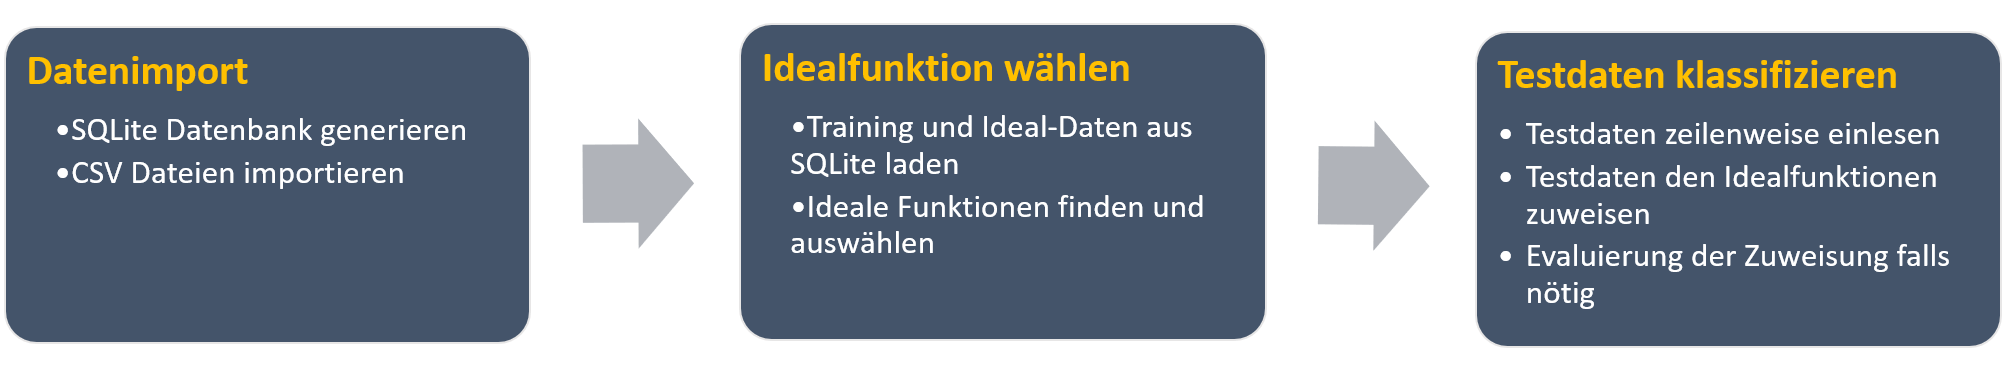
\includegraphics[width=15cm]{pics/Flow.png}\\
Quelle: Eigene Darstellung.
\label{fig:flow}
\end{figure}


\FloatBarrier

\subsection{Installation}
\label{sub:installation}

Für die Installation bietet es sich an, lokal eine virtuelle Pythonumgebung anzulegen. Anschließend kann nach Wechsel in das Projektverzeichnis, mit dem Befehl
\begin{center}\emph{pip install -e .}\end{center}
das Modul \emph{setup.py} ausgeführt und somit das Programm installiert werden. \cite{geer_practical_2019} erläutert zwar in seinem Blog-Post, dass die Verwendung von setup.py mittlerweile eine veraltete Vorgehensweise für die Installation von Projekten darstellt, bietet aber gleichzeitig eine leicht verständliche Anleitung dafür an. Der Autor griff, aus Gründen der Einfachheit, auf diese Beschreibung zurück.  

Mit der Installation werden die Verfügbarkeit der benötigten Dateien überprüft und UnitTests zur Sicherstellung der Funktionalität durchgeführt. Für die Integration der Tests in das Modul setup.py lieferte der Foren-Beitrag von \cite{jesuisme_answer_2021} einen guten Anhalt. Benötigte Pakete werden gegebenenfalls in der virtuellen Umgebung nachinstalliert. Im Rahmen der Installation wird außerdem ein Logfile \emph{setuplog\_[DATUM]\_[UHRZEIT]} im Verzeichnis \emph{output/logs} angelegt. Nach erfolgreicher Installation, kann das Programm aus der Konsole mit dem einfachen Aufruf \emph{\glqq ff\grqq} ausgeführt werden.

Der Konsolenbefehl \emph{python -m unittest -v tests/test\_unit.py} stellt eine detaillierte Ausgabe der Ergebnisse der UnitTests zur Verfügung. 

Im Zuge der Entwicklung wurde das vorliegende Programm mit der Pythonversion 3.11 unter Windows10 getestet. Die Lauffähigkeit auf Linux oder IOS/MacOS Plattformen wurde im gegenständlichen Programmdesign nicht berücksichtigt und bietet sich, aus Sicht des Autors, als Thema für eine Weiterentwicklung der Software an.

\subsection{Konfiguration}

Über Änderungen im Modul \emph{config.py} können, falls benötigt, Verzeichnispfade, Log-Einstellungen, Bewertungsfunktionen, sowie auch die Pfade zu den vorliegenden Datendateien angepasst werden.

Letzteres ermöglicht eine einfache Änderung der verwendeten Trainings-, Funktions- und Testdaten, um das Programm auch mit anderen als den, im Rahmen der Aufgabenstellung, bereitgestellten Daten auszuführen.

Eine Anpassung der Bewertungsfunktionen bietet des weiteren die Möglichkeit, die zur Bewertung der Trainingsdaten herangezogene Funktion (der Standardwert ist hierfür die kleinste Summe der quadratischen Abweichungen) sowie den Faktor für den errechneten Fehlerwert, zur Klassifikation der Testdaten (der Standardwert ist, gemäß Aufgabenstellung, die Wurzel aus Zwei) zu verändern.

\subsection{Dokumentation}

Bei der Dokumentation der Software entschied sich der Autor für eine Formatierung gemäß NumPyDoc Style Guide \citep{numpydoc_v160_style_nodate}. Dieser bietet den Vorteil, durch die Software \emph{Sphinx} automatisiert zu einer übersichtlichen Dokumentation zusammengefasst werden zu können. Die \emph{autosummary}-Funktion von Sphinx ermöglicht hierbei eine rekursive Verarbeitung der in den Modulen, Funktionen und Methoden hinterlegten Dokumentation \citep{leedham_answer_2020}.

Verfügbar ist diese, automatisch generierte, Dokumentation
\begin{itemize}
 \itemsep0pt
 \item als HTML-Website, durch laden der Datei \emph{docs/build/html/index.html}
 \item oder als LATEX-Pdf (\emph{docs/build/latex/dlmdwpmp01.pdf}).
\end{itemize}


\section{Bereitgestellte Datensätze}

\subsection{Beschreibung der Datensätze}

Im Zuge der Aufgabenstellung wurden dem Autor drei Datensätze in Form unten aufgelisteter CSV-Dateien bereitgestellt.

\begin{itemize}
 \itemsep0pt
 \item \emph{train.csv}
 \item \emph{ideal.csv}
 \item \emph{test.csv}
\end{itemize}

Erstere beinhaltet eine Tabelle von vier \glqq verwaschenen\grqq\ mathematischen Funktionen in den Spalten \emph{y1} bis \emph{y4} mit jeweils 400 Datenpunkten. Die folgende Tabelle zeigt die exemplarische Struktur des Trainingsdatensatzes.

\begin{table}[H]
\small
\centering
\caption{Exemplarischer Auszug der Datei train.csv}
\csvautotabular[range={+5}]{../data/train.csv}\\
Quelle: Eigene Darstellung.
\label{tab:train.csv}
\end{table} 


Eine Visualisierung der Trainingsdaten lässt bereits optische Rückschlüsse auf mögliche, passende idealtypische Funktionen zu.

\begin{figure}[h]
\centering
\caption{Darstellung der bereitgestellten Trainingsdatensätze}
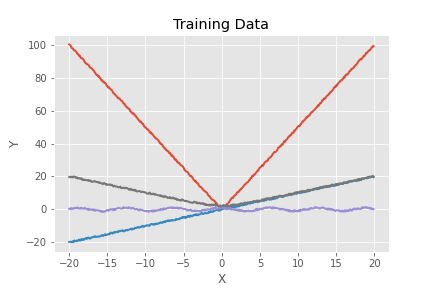
\includegraphics[width=13cm]{../output/figures/train.png}\\
Quelle: Eigene Darstellung.
\label{fig:train}
\end{figure}

Die Datei \emph{ideal.csv} beinhaltet 50, nicht \glqq verwaschene\grqq\ , idealtypische Funktionen in den Spalten \emph{y1} bis \emph{y50}. Wie im Detail im folgenden Abschnitt beschrieben, sollen diese Funktionen durch das Programm mit dem Trainingsdatensatz verglichen werden und daraus die passendsten vier Funktionen gewählt werden. Die Datei weist, bis auf die Anzahl der Spalten, eine ähnliche Struktur wie der Trainingsdatensatz auf und besteht ebenfalls je Spalte aus 400 Datenpunkten. 

\begin{table}[H]
\small
\centering
\caption{Exemplarischer Auszug der Datei ideal.csv}
\csvautotabular[range={+5}]{ideal.csv}\\
Quelle: Eigene Darstellung.
\label{tab:ideal.csv}
\end{table} 

Im Gegenzug zu den oben dargestellten beiden Datensätzen besteht der Testdatensatz nur aus 100 einzelnen Datenpunkten. Diese werden in einer Spalte \emph{y} der Datei \emph{test.csv} zusammengefasst und sind nicht als zusammengehörige Funktion zu verstehen. 

\begin{table}[H]
\small
\centering
\caption{Exemplarischer Auszug der Datei test.csv}
\csvautotabular[range={+5}]{../data/test.csv}\\
Quelle: Eigene Darstellung.
\label{tab:test.csv}
\end{table} 

In der weiteren Bearbeitung der Aufgabenstellung sollen diese Datenpunkte mit den ausgewählten idealtypischen Funktionen verglichen und jeweils jener, mit der geringsten Abweichung, zugewiesen werden. Dieser Vorgang wird im Zuge dieser Arbeit als \glqq Klassifikation der Testdaten\grqq\ bezeichnet und im gleichnamigen Abschnitt im Detail behandelt.

Für die interne Verarbeitung der Daten wurde, im Rahmen des Programms, eine eigene Objektklasse geschaffen, die spezifische Methoden sowie die Parameter der Visualisierung bereitstellt. Diese Klasse und deren Unterklassen für die verschiedenen Datensätze sind im Modul \emph{classes.py} definiert.

\subsection{Ablage der Datensätze in einer SQLite Datenbank}

Gemäß der Vorgabe der Aufgabenstellung sollen sowohl die Trainings- (\emph{train.csv}) als auch die Funktionsdaten (\emph{ideal.csv}) in eine SQLite Datenbank eingelesen werden. Diese wird im Verzeichnis \emph{output/data} bereitgestellt. Der Autor entschied sich hierbei für das Python-Paket \emph{sqlite3} anstelle des, in der Vorgabe vorgeschlagenen, Paketes \emph{sqlalchemy}. Dieses bietet für die gegebene Anwendung eine vereinfachte Möglichkeit Daten mit einer SQLite Datenbank zu verarbeiten \citep{gosset_accessing_2017}.

Über die UnitTests, die im Rahmen der, in Abschnitt ~\ref{sub:installation} beschriebenen, Installation durchgeführt werden, wird unter anderem, das lokale System auf die Möglichkeit eines direkten SQL-Imports hin überprüft. Dies bedeutet, dass versucht wird, die Daten in die SQLite Datenbank zu schreiben, ohne diese zuerst über das Python-Programm einzulesen und erst in einem weiteren Verarbeitungsschritt an die Datenbank zu übergeben. Die Umsetzung hierfür erfolgt nach einem Foren-Beitrag von \cite{stevens-haas_importing_2021} mit dem Paket \emph{subprocess}. Das Ergebnis der Überprüfung wird bei Erfolg im Logfile des Setups angeführt. Auch in der Ausführung des Programms wird vorerst noch einmal der direkte Import versucht und erst im Falle eines Fehlschlages der Umweg über die Methoden des Python-Pakets \emph{pandas} gewählt. Obwohl, aufgrund der geringen Größe, der in dieser Arbeit vorliegenden Datensätze, die Möglichkeit des direkten Imports nur eine untergeordnete Rolle spielt, schont ein solcher, im Falle größerer Datenmengen, die Systemressourcen und spart Zeit in der Programmausführung.

Die Testdaten (\emph{test.csv}) werden, gemäß Vorgabe, in der Programmausführung zeilenweise eingelesen, mit den Daten der gewählten Funktionen verglichen und gemeinsam mit der getroffenen Klassifikation in die SQLite Datenbank geschrieben.


\section{Auswahl idealtypischer Funktionen}

Wie bereits im vorangegangenen Abschnitt angeführt, steht zur Bearbeitung der Aufgabenstellung eine Auswahl an 50 idealtypischen Funktionen in einer CSV-Datei zur Verfügung. Aus diesen sollen, für jede der vier Datenspalten der Trainingsdaten, jeweils die passendste Funktion durch das Programm gewählt werden. Das Kriterium zur Selektion ist, gemäß Aufgabenstellung, die Minimierung der Summe aller quadratischen y-Abweichungen (Least Square).

Mathematisch wird daher der kleinste Wert der Formel
\begin{equation}  
\sum_{i=1}^{n}(TrainingData_{i} - IdealFunction_{i})^2
\label{leastsquare}
\end{equation}
gesucht. Wobei die Variable $TrainingData$ durch alle vier vorliegenden Trainingsdatenspalten iteriert und die Variable $IdealFunction$ durch sämtliche verfügbaren Datenspalten der idealtypischen Funktionen. $n$ steht hierbei für die Anzahl an Datenpunkten je Datenspalte, die, im vorliegenden Programmdesign, in beiden Datensätzen gleichgroß sein muss. Diese Anforderung ist eine wesentliche Voraussetzung für die Funktionalität der Software \emph{functionfinder} und wird bereits im Rahmen der Installation durch einen UnitTest überprüft. Werden die Quelldatensätze nach erfolgter Installation geändert, sollte diese Überprüfung durch eine manuelle Ausführung der UnitTests erfolgen. Die Schaffung einer Toleranz des Programmes gegenüber unterschiedlichen Datensatzgrößen (zB durch statistische Methoden zur Behandlung von fehlenden Werten) wäre, aus Sicht des Autors, eine zielführende Weiterentwicklung des Projekts.

In der Umsetzung des Packages wurde für den mathematischen Teil dieser Aufgabe (gemäß Gleichung ~\ref{leastsquare})  von der Eigenschaft des \emph{pandas}-Objekts \emph{Series} Gebrauch gemacht, die, bei der Subtraktion von zwei gleichlangen \emph{Series} der Länge $n$ (in diesem Fall mit $n=400$) erneut eine \emph{Serie} derselben Länge mit den jeweils subtrahierten Einzelwerten zurück gibt. Auch die mathematische Funktion des Quadrats wird auf jeden Einzelwert der \emph{Serie} angewandt. Die Summenbildung der \emph{Serie} fasst diese nun, dem vorgegebenen Kriterium entsprechend, zu einem Wert zusammen.
Diese Eigenschaft ermöglichte es daher, jede Datenspalte des Trainingsdatensatzes durch die Datenspalten der verfügbaren idealtypischen Funktionen zu iterieren und die zurückgelieferten Ergebnisse direkt zu vergleichen. Das Ergebnis mit der kleinsten Summe wurde jeweils als das Passendste abgespeichert.

Im Programmdesign bot es sich daher an, hierfür zwei Funktionen getrennt zu definieren:
\begin{enumerate}
 \itemsep0pt
 \item Die Funktion der Iteration und des Vergleiches zur Ermittlung des minimalen Fehlers wurde im Modul \emph{datafunctions.py} definiert.
 \item Die Funktion zur Berechnung des Fehlers (gemäß Vorgabe, entsprechend der Gleichung ~\ref{leastsquare}) wurde in der Datei \emph{config.py} definiert.
\end{enumerate}

Dies erlaubt es, auf einfache Weise in der Konfigurationsdatei \emph{config.py}, die Funktion zur Fehlerberechnung zu verändern und gegebenenfalls andere Kriterien, wie zB die durchschnittliche mittlere Abweichung (Mean Squared Error - MSE) zur Bewertung heranzuziehen. 

Als Rückgabewert der ersten genannten Funktion, wurde vom Autor der Python-Datentyp \emph{dictionary} gewählt. In diesem wurde zu jedem \emph{Key} (die Datenspalten des Trainingsdatensatzes) der \emph{Value} in Form eines \emph{Tupels} abgelegt, welcher den Namen der gewählten Datenspalte des Datensatzes idealtypischer Funktionen, sowie die berechnete Abweichung beinhaltet.

\begin{figure}[h]
\caption{Darstellung des Rückgabewertes der berechneten Übereinstimmungen}
\begin{tabular}{l}
\begin{lstlisting}[language=python,label=dictresult]
{'y1': ('y36', 33.71178854422821),
 'y2': ('y11', 32.62893138832121),
 'y3': ('y2', 33.11847188090256),
 'y4': ('y33', 31.75243110139478)}
\end{lstlisting}
\end{tabular}\\
\begin{center}
Quelle: Eigene Darstellung.
\end{center}
\label{fig:resultdict}
\end{figure}

Die oben angeführte Darstellung des Rückgabewertes macht ersichtlich, welche idealtypischen Funktionen für die jeweiligen Trainingsdatenspalten gewählt wurden. Die grafische Repräsentation lässt auch eine optische Bestätigung der getroffenen Auswahl zu.

\begin{figure}[h]
\centering
\caption{Darstellung der ausgewählten idealtypischen Funktionen}
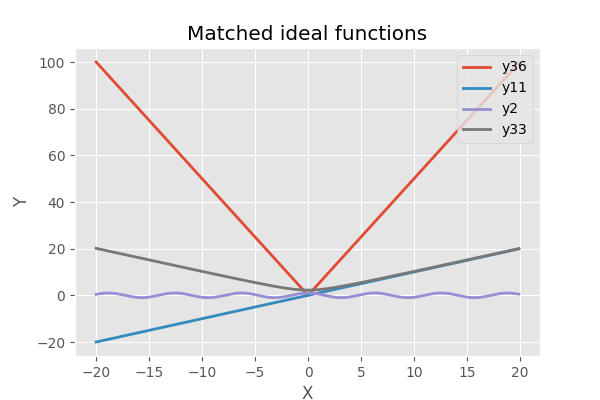
\includegraphics[width=13cm]{../output/figures/ideal.png}\\
Quelle: Eigene Darstellung
\label{fig:ideal}
\end{figure}

\section{Klassifikation der Testdaten}
\label{sec:class}

In diesem Abschnitt wird die Klassifikation der Testdaten mithilfe der ausgewählten idealtypischen Funktionen sowie den jeweiligen berechneten Abweichungen (siehe vorangegangener Abschnitt) diskutiert.

Entsprechend der Vorgabe zur vorliegenden Aufgabenstellung werden die, in der Datei \emph{test.csv}, abgebildeten Datenpunkte, Zeile für Zeile eingelesen und mit dem maximalen Abstand von $ a*\sqrt{2}$ einer der vier gewählten Funktionen zuordnet. Wobei $a$ den berechneten Fehlerwert des Trainingsdatensatzes der jeweiligen Funktion repräsentiert. Hierbei unterstützt das Paket \emph{csv} den Vorgang der zeilenweisen Iteration \citep{python_software_foundation_csv_nodate-1}.

In der Umsetzung wurde die oben angeführte Berechnungsformel wiederum in zwei Teile gegliedert. Der Wert $a$ stammt aus einer vorangegangenen Berechnung und ist an dieser Stelle bereits bestimmt. Der zweite Teil betrifft den Multiplikationsfaktor $\sqrt{2}$, der durch die Vorgabe zur Aufgabenstellung festgelegt wurde. Um diesen gegebenenfalls anpassen zu können wurde dazu die Variable \emph{factor} in der Konfigruationsdatei \emph{config.py} definiert. Dadurch wird wiederum eine flexible Herangehensweise an die Bewertung der Testdaten gewährleistet.

Für die Bewertung selbst wurde im Modul \emph{datafunctions.py} die Funktion \emph{calculate\_best\_ideal} definiert. Diese nimmt im Wesentlichen als Parameter die aktuell eingelesene Zeile der Datei \emph{test.csv}, die Auswahl der idealtypischen Funktionen inklusive der Fehlerberechnungen, den Datensatz der idealtypischen Funktionen, sowie einen Funktionsparameter für die Filterung der Ergebnisse entgegen. 

Letzterer ist für die Berechnung der passenden idealtypischen Funktion auf \emph{min} gesetzt. Das bedeutet, dass aus den Abweichungen zu allen vier gewählten Funktionen, diejenige mit der kleinsten Abweichung gewählt wird.

Das zeilenweise Einlesen der Testdaten könnte, im Fall der Bearbeitung größerer Datenmengen die Prozessdauer des Programmes negativ beeinflussen. Das \emph{pandas} Paket bietet die Möglichkeit die oben angeführte Funktion auf jede Observation eines Objektes vom Typ DataFrame anzuwenden. Hierdurch würde, in diesem Fall, eine vermeintliche Steigerung der Performance erzielt, wenn der Testdatensatz in Gänze als \emph{DataFrame} bearbeitet würde. Die Struktur des veränderten \emph{DataFrame} entspräche durch die funktionale Erweiterung dem geforderten Ergebnis. Ein solches Vorgehen würde allerdings eine Abweichung der Vorgabe der zeilenweisen Bearbeitung bedingen und wäre, aus Sicht des Autors in einer weiterführenden Arbeit zu evaluieren.   

Die Aufgabenstellung sieht vor, dass die Testdaten um die Werte der Abweichung (DeltaY), sowie die Nummer der gewählten Funktion (Idealfunktion) erweitert werden und in eine eigene Tabelle der SQLite Datenbank geschrieben werden. Der Autor entschied sich an dieser Stelle, noch einen Wert (Off\_limit) hinzuzufügen. Dieser Wert, vom Datentyp \emph{Boolean}, zeigt an, wenn dieser Datenpunkt den gesetzten Maximalabstand ($a*\sqrt{2}$) zu keiner der gewählten Funktionen einhalten konnte und wird in diesem Fall auf \emph{True} gesetzt. Dem Datenpunkt wird aber dennoch die Funktion mit dem geringsten Abstand zugewiesen. Der nachfolgende exemplarische Auszug der Ergebnisse aus der Tabelle \emph{test} der SQLite Datenbank zeigt die angesprochene Struktur der ausgegebenen Daten. In der letzten Datenreihe wird auch ersichtlich, dass dieser Datenpunkt den angeführten Maximalabstand bei keiner, der gewählten idealtypischen Funktionen, einhalten konnte. Die Zuweisung ist daher so zu verstehen, dass in diesem Fall die Funktion \emph{y36} den geringsten Abstand zu diesem Datenpunkt aufwies.

\begin{table}[H]
\small
\centering
\caption{Exemplarischer Auszug der Ergebnisse aus der SQLite Datenbank}
\csvautotabular[range={+5}]{sqlitetest.csv}\\
Quelle: Eigene Darstellung.
\label{tab:sqlitetest.csv}
\end{table} 

Für eine Evaluierung der Ergebnisse wurde in der Objektklasse \emph{testdata} die Methode \emph{off\_limit} definiert, die aus der SQLite Datenbank jene Werte abfrägt, bei denen dieser Wert auf \emph{True} gesetzt ist. Diese Datenpunkte werden nochmals an die Funktion \emph{calculate\_best\_ideal} übergeben, wobei diesmal der Funktionsparameter für die Filterung auf \emph{raw} gesetzt wird. Dadurch werden die Ergebnisse des Vergleichs zu jeder der vier gewählten idealtypischen Funktionen ausgegeben und können über das Logfile manuell evaluiert werden.

Bei der Bearbeitung der zur Aufgabe übergebenen Datensätze waren hierbei zwei Datenpunkte des Testdatensatzes betroffen. Der aufbereitete Auszug aus dem entsprechenden Logfile zeigt die unten angeführten Ergebnisse:

\begin{figure}[h]
\caption{Datenpunkte mit überschrittenem Maximalabstand}
\begin{tabular}{l}
\begin{lstlisting}[label=offlimit]
/  2 entries had a deviation above the set limit:

|  x         y     DeltaY Idealfunktion  Off_limit
/ -6.5  81.21402  48.714020           y36       True
| -6.5  81.21402  87.714020           y11       True
| -6.5  81.21402  80.237432            y2       True
| -6.5  81.21402  74.340156           y33       True

|  x         y     DeltaY Idealfunktion  Off_limit
| 0.3  59.68033  58.180330           y36       True
| 0.3  59.68033  59.380330           y11       True
| 0.3  59.68033  58.724993            y2       True
/ 0.3  59.68033  57.424227           y33       True
\end{lstlisting}
\end{tabular}\\
\begin{center}
Quelle: Eigene Darstellung.
\end{center}
\label{fig:offlimit}
\end{figure}

In den oben angeführten Tabellen wird die Distanz der beiden betroffenen Datenpunkte zu allen vier gewählten Funktionen ersichtlich. In der Zuweisung wurden dennoch jene Funktionen mit dem geringsten Abstand gewählt (grafisch hervorgehoben).

In der grafischen Repräsentation der Ergebnisse ist die Annäherung der einzelnen Datenpunkte des Testdatensatzes an die gewählten idealtypischen Funktionen gut erkennbar. Jene beiden Datenpunkte, die im Vergleich den definierten Maximalabstand überschritten haben werden durch das Symbol $x$ dargestellt und liegen etwa bei den Koordinaten (-7/81) sowie (0/60). Wobei hier die optische Beurteilung des zweiten Punktes eher eine Tendenz zur Funktion \emph{y36} vermuten ließe, als zur Funktion \emph{y33}. In der oben angeführten Darstellung zu diesem Datenpunkt wird aber auch deutlich, dass die berechneten Abstände tatsächlich sehr nahe beieinander liegen.

Würde die Distanz allerdings unter dem Aspekt der Relation zur berechneten Abweichung betrachtet werden, entspräche die Klassifikation der oben angesprochenen, optischen Beurteilung, wie die nachfolgenden Berechnungen veranschaulichen. Hier liefert der zweite Wert, mit der größeren Punktabweichung, einen geringeren relativen Abweichungswert und würde daher bei einer Klassifikation unter diesem Aspekt herangezogen werden. 

\begin{center}
y33: $ \frac{57.424227\ (Punktabweichung)}{31.752431\ (Fehlerwert\ Funktion\ y33)} = 1.808498 $ 
\end{center}

\begin{center}
y36: $ \frac{58.180330\ (Punktabweichung)}{33.711788\ (Fehlerwert\ Funktion\ y36)} = 1.725815 $
\end{center}

Diese \glqq Normalisierung\grqq\ der Abweichung und damit eine Klassifikation in Relation zum berechneten Fehlerwert $a$ jeder ausgewählten idealtypischen Funktionen, könnte gerade in Grenzfällen, wie diesem, einen Unterschied in der Zuweisung hervorrufen. Aus Sicht des Autors, zeichnet sich hierbei eine mögliche Weiterentwicklung des Programmes ab, die jedoch zuvor durch einen Vergleichstest evaluiert werden sollte.

Wie anhand der Visualisierung jedoch beobachtet werden kann, liefert auch eine Klassifikation, ohne der oben angesprochenen Modifikation, an den Schnittpunkten der Funktionen eine ausreichend gute Zuweisung. Der Verlauf der idealtypischen Funktionen kann hier auch in den Testdaten optisch nachverfolgt werden.

\begin{figure}[h]
\centering
\caption{Klassifikation der Testdatensätze}
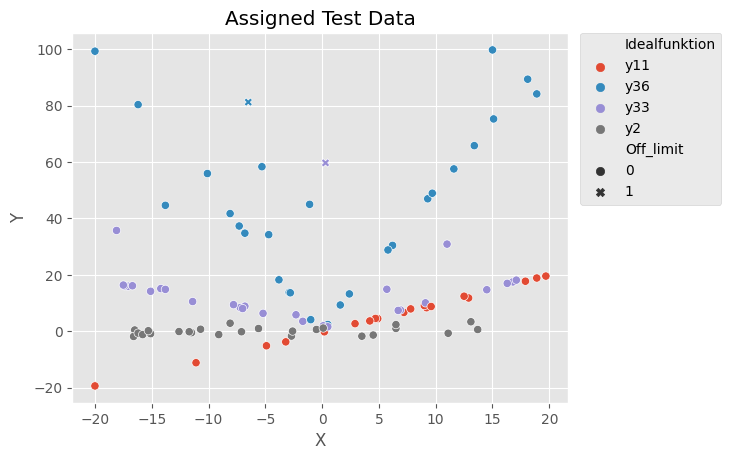
\includegraphics[width=13cm]{../output/figures/test.png}\\
Quelle: Eigene Darstellung
\label{fig:test}
\end{figure}


\chapter{Zusammenfassung}

Wie Eingangs erwähnt, wird an dieser Stelle noch einmal betont, dass bei der Bearbeitung der gegenständlichen Aufgabenstellung in erster Linie die Erlernung des Umgangs mit der Programmiersprache Python im Vordergrund stand. Für den Autor war hierbei der exemplarische Aufbau und die Struktur eines selbst erstellten Pythonpackages, sowie das Zusammenspiel und die Anpassungsfähigkeit der einzelnen Skripte von besonderer Bedeutung.

Es wurde hierbei versucht, die Vorgaben der Aufgabenstellung weitestgehend zu erfüllen. Wie jedoch bereits in den vorangegangenen Abschnitten erläutert, waren aus Sicht des Autors, zwei Modifikationen der Software bereits in der ersten Umsetzung sinnvoll.
\begin{enumerate}
 \itemsep0pt
 \item  Der automatisierte Versuch des \emph{direkten} Imports der Daten in die SQLite Datenbank.
 \item  Die Erweiterung der verfügbaren Datenspalten des Ergebnisses der klassifizierten Testdaten.
\end{enumerate}
Die erstgenannte Anpassung begünstigt, bei gegebenen Systemvoraussetzung die Verarbeitung größerer Quelldatensätze.
Die Zweite lässt eine Ausgabe jener Ergebnisse zu, die den vorgegebenen Maximalabstand zu keiner der ausgewählten idealtypischen Funktionen einhalten konnten.

Des Weiteren wurden, im Rahmen dieser Arbeit, Themenbereiche angesprochen, die mögliche Ansätze für eine Weiterentwicklung des Programmes darstellen:

\begin{enumerate}
 \itemsep0pt
 \item Zur Sicherstellung der Lauffähigkeit der Software auf unterschiedlichen Betriebssystemen, gab es im Zuge der Aufgabenstellung keine Vorgaben. Um jedoch das Testen der Software zu erleichtern, wäre eine plattformunabhängige Version des Progammes, aus Sicht des Autors, sinnvoll.
 \item In der Aufgabenstellung wurden exakt zugeschnittene Quelldatensätze zur Verfügung gestellt. In Fällen wo solche \glqq Laborbedingungen\grqq\ jedoch nicht zutreffen, würde die Schaffung einer Toleranz der Software gegenüber unterschiedlichen Datensatzgrößen der Trainings- und idealtypischen Funktionsdaten die Resilienz des Programmes erhöhen.
 \item Bei Vorlage eines größeren Testdatensatzes, wäre eine tabellenweise Verarbeitung, nach Meinung des Autors, performanter als die vorgegebene zeilenweise Kalkulation.
 \item Wie in Abschnitt ~\ref{sec:class} erläutert, könnte eine \glqq Normalisierung\grqq\ des kalkulierten Abstandswertes zur Klassifikation in Relation zum zuvor berechneten Fehlerwert der idealtypischen Funktion, die Klassifikation in Grenzfällen positiv beeinflussen. Eine solche Modifikation sollte jedoch, aus Sicht des Autors, zuvor getestet und evaluiert werden.
\end{enumerate}

Oben genannte Anpassungen kämen der Resilienz der Software, der Effizienz des Programmes in der Verarbeitung größerer Datensätze, sowie der Genauigkeit der Klassifikation der Testdaten zugute. Eine Validierung dieser Annahmen wäre, aus Sicht des Autors, eine mögliche Fragestellung für eine weiterführende Arbeit. 


